\documentclass[11pt]{article}

\usepackage[margin=1in]{geometry}
\usepackage{amsmath,amssymb,amsthm}
\usepackage{hyperref}
\usepackage{float}
\usepackage{graphicx}
\usepackage{booktabs}
\usepackage{subcaption}
\usepackage{longtable}
\usepackage{fontspec}
\usepackage{tikz}
\usetikzlibrary{arrows.meta, backgrounds, calc, fit, positioning}

\tikzset{
  rtarrow/.style={->, >=Stealth, thick},
  rtlatent/.style={circle, draw, thick, minimum size=18pt, inner sep=1pt},
  rtobs/.style={rtlatent, fill=gray!20},
  rtconst/.style={rectangle, draw, thick, rounded corners, inner sep=2pt, minimum height=16pt},
  rtplate/.style={draw, rounded corners, dashed, inner sep=6pt},
}

\setmainfont{Times New Roman}
\setmonofont[Scale=0.9]{Menlo}

% Render code-like identifiers without oversized monospace.
\newcommand{\codeword}[1]{\textnormal{\detokenize{#1}}}

\graphicspath{{./}{images/}{images/rt_pymc_multilevel_pooling_report/}{docs/models/}{docs/models/images/}{docs/models/images/rt_pymc_multilevel_pooling_report/}}

\setlength{\parindent}{0pt}
\setlength{\parskip}{0.7\baselineskip}

\title{Report: RT Regression Model (Hierarchical Ridge with Chemistry)}
\author{Bioinformatics Team}
\date{\today}

\begin{document}

\maketitle

\section{Introduction}

Sally is Metabolon’s production autocuration system for LC--MS peak assignment. For each sample set (SSID), it processes
many LC tasks and determines, for each library compound, whether the compound is present and (if so) which observed peak
best matches that compound. Within a single task, mass-based matching can produce multiple plausible candidate peaks, so
Sally relies on additional evidence to reject decoys and to select the best remaining peak.

Retention time (RT) is a key signal in this decision. For each (task, compound) pair, Sally uses an RT regression model
to predict an expected RT, \codeword{expectedRT}. It also attaches a window half-width, \codeword{expectedRTWindow}.
Candidate peaks are filtered by this window:
\[
  \lvert \text{apex\_rt} - \text{expectedRT} \rvert \le \text{expectedRTWindow}.
\]
If multiple peaks remain for the same compound in a task, Sally chooses the peak closest to the predicted RT after
applying a per-compound correction factor (the median RT shift across tasks within the SSID), and then removes
outliers with a small fixed buffer around the corrected center. Because RT enters as a hard filter, the RT window is
operationally important: windows that are too narrow remove true peaks (false negatives), while windows that are too wide
allow decoys to survive and can increase false positives.

In current production, \codeword{expectedRT} comes from a bank of supercategory-specific lasso regression models
(\codeword{ESLASSO}). Models are partitioned by \codeword{species_matrix_type} (called \texttt{species\_cluster} in this
report) and trained independently for each library compound using run-level covariates derived from internal standards
(the \texttt{IS*}/\texttt{RS*}/\texttt{ES\_\*} columns). Each compound model stores point-estimate coefficients and a fixed
per-compound RT window derived from held-out residual variation; at scoring time the window is scaled by a global
\codeword{windowMultiplier} and clamped to a minimum width. This design is practical and fast, and it captures broad
matrix-specific RT structure and run drift. However, it is brittle in sparse settings: rare species and infrequently
observed compounds receive limited statistical sharing, and the $\ell_1$ penalty can behave poorly under correlated run
covariates, leading to unstable coefficients across retrains. Moreover, fixed windows are heuristic and do not provide a
calibrated predictive distribution, making it difficult to reason about coverage and filtering trade-offs systematically.

This report replaces the lasso baseline with a hierarchical Bayesian ridge regression with chemistry-informed sharing.
The model partially pools species effects within each supercategory, regularizes compound baselines toward a
chemistry-derived prior mean (from ChemBERTa embeddings), and uses ridge shrinkage to stabilize correlated run covariates.
It yields a predictive distribution for RT, which we convert to task-specific RT windows for filtering. To keep training
tractable at production scale, we analytically collapse the per-group slopes and fit the remaining hierarchy with
variational inference. For deployment, we export compact stage-1 coefficient summaries so that Sally can score
deterministically at runtime without running Bayesian inference.

Finally, RT evidence is often strongest when aggregated across tasks. A false positive can survive the per-task RT window
filter yet form an implausible across-task RT pattern for a compound. We therefore introduce an SSID-specific coherence
check (\codeword{peak_assignment_method} = \codeword{mixture_model}) based on a two-component Bayesian Gaussian mixture fitted to
per-compound mean RT log-likelihoods. The posterior probability of belonging to the coherent component provides a
continuous, data-adaptive criterion for rejecting likely false positives without a fixed global threshold.

We evaluate both offline RT metrics and end-to-end peak assignment performance on held-out test sample sets, comparing the
hierarchical model and coherence check against the production baseline.

\section{Methods}

This section describes the proposed RT model (hierarchical ridge with chemistry), the coherence check used for
across-task rejection, and the baselines used for comparison. We start with a high-level decomposition and then give a
complete probabilistic specification (likelihood, priors, and inference), followed by the production peak-assignment
procedure that consumes RT predictions.

\subsection{Data and notation}

Each RT observation row $i$ contains:
\begin{itemize}
  \item response $y_i$ (RT, minutes),
  \item run covariates $x_{i,j}$ for $j=1,\ldots,p$ from numeric \texttt{IS*}/\texttt{RS*}/\texttt{ES\_\*} columns,
  \item identifiers: \texttt{species\_cluster} $s(i)$, \texttt{species} $c(i)$, \texttt{comp\_id} $k(i)$.
\end{itemize}
In this report, \texttt{species\_cluster} corresponds to the production ``supercategory'' (matrix) grouping used to
partition models in the baseline.

Each compound id $k$ maps to a chemical identifier $h(k)$ (\texttt{compound}/\texttt{chem\_id}), which has a fixed
ChemBERTa PCA-20 embedding $e_{h(k),d}$ for $d=1,\ldots,D$ (with $D=20$). ChemBERTa is a pretrained transformer model
that reads SMILES strings (a text representation of chemical structure) and produces vector embeddings where chemically
similar compounds tend to have similar representations. We use these embeddings to let the model share information
across compounds when direct training support for a compound is sparse. The embeddings are built offline from SMILES
strings using the pretrained ChemBERTa encoder and then projected to 20 dimensions with PCA for compactness; in this
model they are treated as fixed inputs.

For numerical stability we treat the run covariates as globally centered
($x_{i,j}\leftarrow x_{i,j} - \bar{x}_{j,\text{train}}$ for each $j$). This is a pure reparameterization in a linear
model with an intercept: it does not change the underlying fit, but it reduces intercept--slope coupling and improves
conditioning.

\subsection{High-level model decomposition}

We model RT as:
\[
  \text{RT} \;=\; \underbrace{\text{(species + compound baseline)}}_{\text{intercept}} \;+\;
  \underbrace{\text{(run adjustment)}}_{\text{slopes on run covariates}} \;+\;
  \underbrace{\text{noise}}_{\text{residual RT variation}}.
\]

Concretely, each (species, compound) pair defines a group
\[
  g = (c, k) = (\texttt{species}, \texttt{comp\_id}),
\]
and we fit one linear regression per group:
\[
  y_i = b_{g(i)} + \sum_{j=1}^{p} x_{i,j}\,w_{g(i),j} + \epsilon_i,\qquad
  \epsilon_i \sim \mathcal{N}(0,\sigma^2).
\]

The model becomes useful in the long tail because we do \emph{not} fit each $b_{c,k}$ and $w_{c,k,1:p}$ independently:
we place hierarchical (partially pooled) priors on intercepts and slope means, and we tie compound effects to chemistry.

\subsection{Model specification (at a glance)}

For reference, this section summarizes the full generative model by separating observed quantities, the likelihood, and
priors. We also spell out the indexing to make clear what is shared across supercategories, species, compounds, and
observations.

We use the following indices and mappings:
\begin{itemize}
  \item observation index $i \in \{1,\ldots,N\}$ for RT rows,
  \item run-covariate index $j \in \{1,\ldots,p\}$,
  \item supercategory index $s$ (production \texttt{species\_cluster}),
  \item species index $c$ (nested in a supercategory),
  \item compound index $k$ (\texttt{comp\_id}),
  \item chemical id $h=h(k)$ (\texttt{chemical\_id}),
  \item embedding dimension $d \in \{1,\ldots,D\}$ (with $D=20$).
\end{itemize}
Row $i$ belongs to a group $g(i)=(c(i),k(i))$ and to a supercategory $s(i)$. The mapping $s(c)$ returns the
supercategory containing species $c$, and the mapping $h(k)$ returns the chemical id for compound $k$. For chemistry,
$z_{h,d}=e_{h,d}-\bar{e}_{d,\text{train}}$ denotes the centered ChemBERTa embedding for chemical id $h$.

We observe $(y_i, x_{i,1:p}, s(i), c(i), k(i))$ for $i=1,\ldots,N$, and we treat centered ChemBERTa embeddings
$z_{h(k),1:D}$ as fixed inputs. Hyperparameters such as $\lambda_{\mathrm{slopes}}$ and prior scales
($\sigma_{\bullet}$) are fixed.

The main model parameters are:
\begin{itemize}
  \item $\sigma_y$: global residual noise scale for RT (shared across all observations),
  \item $t_0$: global RT baseline (supercategory-wide intercept),
  \item $\mu_s$: supercategory-level intercept offset, and $\mu_c$: species-level offset within supercategory,
  \item $\alpha_k$: compound baseline effect (shared across species) with a chemistry-informed prior mean,
  \item $b_{c,k}$: group intercept for each (species, compound) pair, which combines $t_0$, $\mu_c$, and $\alpha_k$,
  \item $w_{c,k,1:p}$: group slopes for run covariates (per (species, compound)), centered around hierarchical means,
  \item $w_0$, $m_s$, $m_c$: global, supercategory, and species slope means, respectively,
  \item $\tau$ scale parameters (e.g.\ $\tau_{\mu,s}$, $\tau_{w,s}$, $\tau_{\mathrm{comp}}$, $\tau_b$) that control the
  strength of partial pooling (smaller $\tau$ means stronger shrinkage toward the parent level).
\end{itemize}

These parameters are shared at different levels:
\begin{itemize}
  \item global: $t_0$, $\sigma_y$, $w_{0,1:p}$, $\theta_{\alpha,1:D}$, $\lambda_{\mathrm{slopes}}$, and the scale
  parameters $\tau_{\mu,\mathrm{supercat}}$, $\tau_{w,\mathrm{supercat}}$, $\tau_{\mathrm{comp}}$, and $\tau_b$,
  \item per-supercategory: $\mu_s$, $m_{s,1:p}$, $\tau_{\mu,s}$, and $\tau_{w,s}$,
  \item per-species: $\mu_c$ and $m_{c,1:p}$,
  \item per-compound: $\alpha_k$ (with residual $\delta_k$),
  \item per-(species, compound) group: $b_{c,k}$ and $w_{c,k,1:p}$.
\end{itemize}

For each row $i$, we model the observed RT $y_i$ as a noisy observation of a group-specific linear predictor. The group
is the (species, compound) pair $g(i)=(c(i),k(i))$, and $w_{g(i),j}$ are the group slopes on centered run covariates
$x_{i,j}$. Conditional on the group coefficients, observations are independent.

\begin{subequations}
\label{eq:rt_pp_ridge_model}
{\small
\begin{align}
  y_i \mid b_{g(i)}, w_{g(i),1:p}, \sigma^2 &\sim \mathcal{N}\!\left(
    b_{g(i)} + \sum_{j=1}^{p} x_{i,j}\,w_{g(i),j}, \sigma^2
  \right). \label{eq:rt_pp_ridge_lik}
\end{align}
}

We assume a single residual noise scale $\sigma_y$ shared across all observations. We use a HalfNormal prior to enforce
positivity and to discourage implausible noise values. We write $\sigma^2=\sigma_y^2$ for convenience.

{\small
\begin{align}
  \sigma_y &\sim \mathrm{HalfNormal}(\sigma_{y,\mathrm{prior}}), \qquad \sigma^2 = \sigma_y^2.
  \label{eq:rt_pp_ridge_noise}
\end{align}
}

We model systematic baseline RT differences across supercategories and species using additive offsets. Each supercategory
has an offset $\mu_s$, and each species has an offset $\mu_c$ that is shrunk toward its supercategory mean $\mu_{s(c)}$.
This implements partial pooling: species with little data are pulled toward the supercategory mean. We allow each
supercategory to have its own pooling strength through $\tau_{\mu,s}$. In implementation we center these offsets to have
mean zero so that $t_0$ remains the overall RT baseline.

{\small
\begin{equation}
\begin{aligned}
  \tau_{\mu,\mathrm{supercat}} &\sim \mathrm{HalfNormal}(\sigma_{\tau_\mu}), \\
  \tau_{\mu,s} &\sim \mathrm{HalfNormal}(\sigma_{\tau_\mu}), \\
  \mu_s \mid \tau_{\mu,\mathrm{supercat}} &\sim \mathcal{N}(0, \tau_{\mu,\mathrm{supercat}}^2), \\
  \mu_c \mid \mu_{s(c)}, \tau_{\mu,s(c)} &\sim \mathcal{N}(\mu_{s(c)}, \tau_{\mu,s(c)}^2).
\end{aligned}
\label{eq:rt_pp_ridge_species_offsets}
\end{equation}
}

The compound effect $\alpha_k$ is decomposed into a chemistry-driven prior mean plus a residual. The embedding weights
$\theta_{\alpha,1:D}$ learn a global mapping from ChemBERTa space to RT baselines, and $\delta_k$ allows each compound to
deviate from the chemistry-predicted mean when the data support it. The residual scale $\tau_{\mathrm{comp}}$ controls
how strongly we trust the chemistry prior mean.

Chemistry only helps when a compound can be mapped from \texttt{comp\_id} to a \texttt{chem\_id} with a ChemBERTa
embedding (derived from a SMILES string). When this mapping or embedding is missing, we fall back to the mean embedding;
after centering, this is equivalent to setting $z_{h(k),1:D}=0$, so the chemistry-derived part of $\alpha_k$ is $0$. In
that case, compounds seen in training can still deviate through the residual $\delta_k$, while unseen compounds have a
zero chemistry backoff.

{\small
\begin{equation}
\begin{aligned}
  \tau_{\mathrm{comp}} &\sim \mathrm{HalfNormal}(\sigma_{\tau_{\mathrm{comp}}}), \\
  \theta_{\alpha,d} &\sim \mathcal{N}(0, \sigma_\theta^2), \qquad d=1,\ldots,D, \\
  \delta_k \mid \tau_{\mathrm{comp}} &\sim \mathcal{N}(0, \tau_{\mathrm{comp}}^2), \\
  \alpha_k &= \sum_{d=1}^{D} z_{h(k),d}\,\theta_{\alpha,d} + \delta_k.
\end{aligned}
\label{eq:rt_pp_ridge_chemistry}
\end{equation}
}

The intercept $b_{c,k}$ is the baseline RT for compound $k$ in species $c$. We draw it around the additive baseline
$t_0 + \mu_c + \alpha_k$ with residual scale $\tau_b$, which captures remaining between-(species, compound) variation not
explained by the species and compound terms.

{\small
\begin{equation}
\begin{aligned}
  t_0 &\sim \mathcal{N}(0, \sigma_{t0}^2), \\
  \tau_b &\sim \mathrm{HalfNormal}(\sigma_{\tau_b}), \\
  b_{c,k} \mid t_0, \mu_c, \alpha_k, \tau_b &\sim \mathcal{N}(t_0 + \mu_c + \alpha_k, \tau_b^2).
\end{aligned}
\label{eq:rt_pp_ridge_intercepts}
\end{equation}
}

Run covariates (e.g., internal-standard intensities) shift RT, and these effects can vary by species. We model this by
placing hierarchical priors on slope means: a global mean $w_{0,j}$, a supercategory mean $m_{s,j}$, and a species mean
$m_{c,j}$. This is another form of partial pooling: species slope means are pulled toward their supercategory means, which
stabilizes estimates for rare species and for correlated covariates.

{\small
\begin{equation}
\begin{aligned}
  \tau_{w,\mathrm{supercat}} &\sim \mathrm{HalfNormal}(\sigma_{\tau_w}), \\
  \tau_{w,s} &\sim \mathrm{HalfNormal}(\sigma_{\tau_w}), \\
  w_{0,j} &\sim \mathcal{N}(0, \sigma_{w0}^2), \qquad j=1,\ldots,p, \\
  m_{s,j} \mid w_{0,j}, \tau_{w,\mathrm{supercat}} &\sim \mathcal{N}(w_{0,j}, \tau_{w,\mathrm{supercat}}^2), \\
  m_{c,j} \mid m_{s(c),j}, \tau_{w,s(c)} &\sim \mathcal{N}(m_{s(c),j}, \tau_{w,s(c)}^2).
\end{aligned}
\label{eq:rt_pp_ridge_slope_means}
\end{equation}
}

Within each (species, compound) group, the slope $w_{c,k,j}$ is shrunk toward the species mean $m_{c,j}$ with strength
controlled by $\lambda_{\mathrm{slopes}}$ (larger values mean stronger shrinkage). We use a ridge (Gaussian) prior
because run covariates are often highly correlated: ridge shrinkage tends to distribute weight smoothly across
correlated predictors and gives more stable fits, whereas lasso-style sparsity can arbitrarily pick one covariate and
lead to unstable coefficients.

{\small
\begin{equation}
  w_{c,k,j} \mid m_{c,j}, \sigma^2, \lambda_{\mathrm{slopes}} \sim \mathcal{N}(m_{c,j}, \sigma^2/\lambda_{\mathrm{slopes}}),
  \qquad j=1,\ldots,p.
\label{eq:rt_pp_ridge_slopes}
\end{equation}
}
\end{subequations}

\subsection{Generative process}

Conditioned on fixed inputs $(x_{i,1:p}, z_{h,1:D})$, the model defines a generative process: it specifies a
step-by-step way one could simulate RT observations by drawing parameters and then generating $y_i$.
\begin{itemize}
  \item draw global scales and baselines ($\sigma_y, t_0, w_{0,1:p}$) and chemistry weights $\theta_{\alpha,1:D}$,
  \item for each supercategory $s$, draw offsets and slope means ($\mu_s, m_{s,1:p}$),
  \item for each species $c$, draw offsets and slope means around its supercategory ($\mu_c, m_{c,1:p}$),
  \item for each compound $k$, compute a chemistry-informed baseline $\alpha_k$,
  \item for each (species, compound) pair $(c,k)$, draw group coefficients $(b_{c,k}, w_{c,k,1:p})$,
  \item for each observation $i$, generate $y_i$ from a Normal distribution with mean
  $b_{g(i)} + \sum_{j} x_{i,j} w_{g(i),j}$ and variance $\sigma^2$.
\end{itemize}

We assume RT is an additive linear function of run covariates plus noise, and that observations are independent once we
condition on the group coefficients. We use one shared noise scale $\sigma_y$. Hierarchical priors provide the main
information sharing: species offsets and slope means are pulled toward their supercategory means, with the $\tau$ pooling
scales controlling how strong that pooling is. For slopes we use a ridge (Gaussian) prior so correlated run covariates
behave stably. Chemistry enters only through $\alpha_k$: embeddings define a prior mean, and $\delta_k$ allows the data
to override that mean when there is enough support.

\begin{figure}[H]
\centering
\small
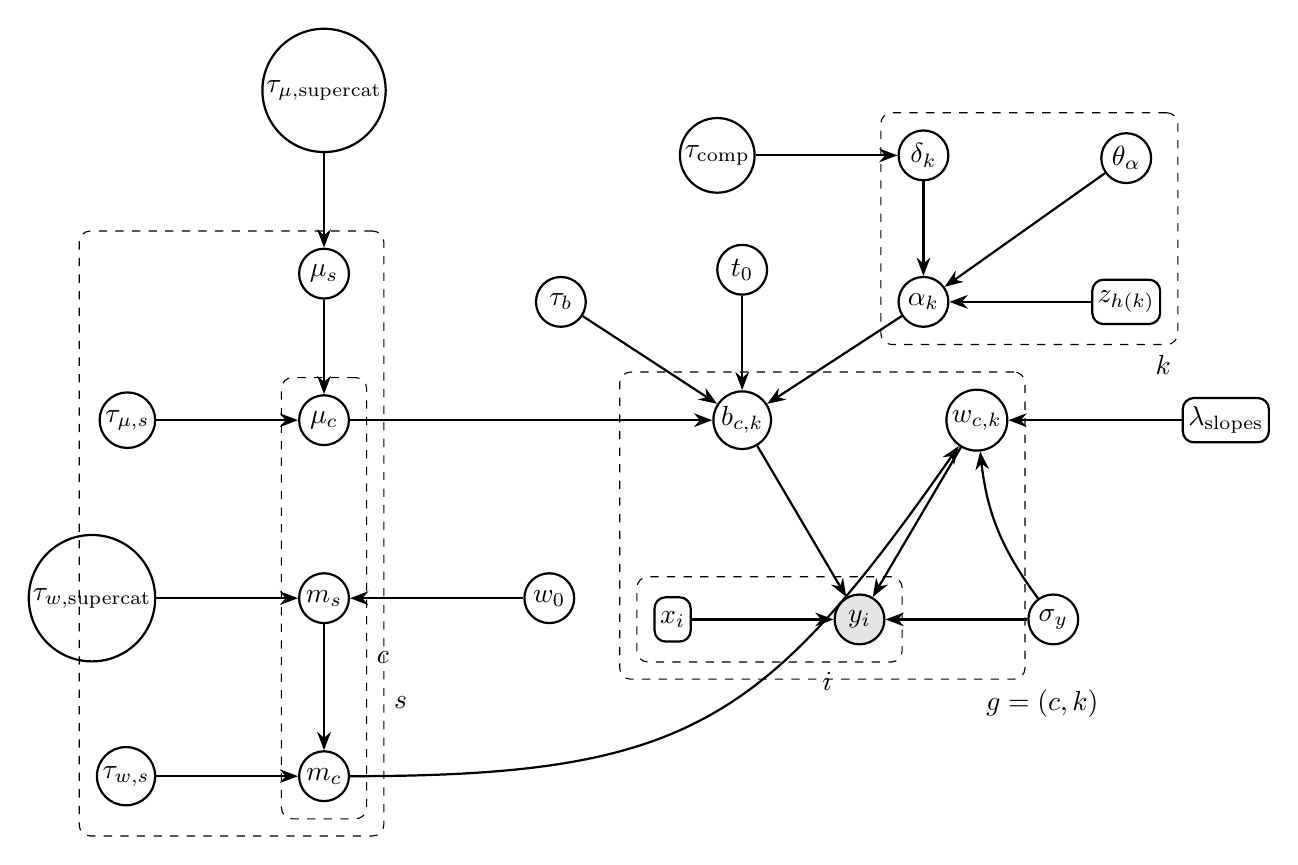
\begin{tikzpicture}
  % Species / supercategory hierarchy (intercepts + slope means).
  \node[rtlatent] (mu_s) {$\mu_s$};
  \node[rtlatent, below=12mm of mu_s] (mu_c) {$\mu_c$};
  \node[rtlatent, above=12mm of mu_s] (tau_mu_sc) {$\tau_{\mu,\mathrm{supercat}}$};
  \node[rtlatent, left=18mm of mu_c] (tau_mu_s) {$\tau_{\mu,s}$};

  \node[rtlatent, below=16mm of mu_c] (m_s) {$m_s$};
  \node[rtlatent, below=16mm of m_s] (m_c) {$m_c$};
  \node[rtlatent, left=18mm of m_s] (tau_w_sc) {$\tau_{w,\mathrm{supercat}}$};
  \node[rtlatent, left=18mm of m_c] (tau_w_s) {$\tau_{w,s}$};
  \node[rtlatent, right=22mm of m_s] (w0) {$w_0$};

  % Group-level coefficients (per (species, compound)).
  \node[rtlatent, right=46mm of mu_c] (b) {$b_{c,k}$};
  \node[rtlatent, right=22mm of b] (w) {$w_{c,k}$};
  \node[rtlatent, above=12mm of b] (t0) {$t_0$};
  \node[rtlatent, above left=10mm and 18mm of b] (tau_b) {$\tau_b$};
  \node[rtconst, right=22mm of w] (lambda) {$\lambda_{\mathrm{slopes}}$};

  % Chemistry-informed compound effects.
  \node[rtlatent, above right=10mm and 18mm of b] (alpha) {$\alpha_k$};
  \node[rtlatent, above=12mm of alpha] (delta) {$\delta_k$};
  \node[rtlatent, left=18mm of delta] (tau_comp) {$\tau_{\mathrm{comp}}$};
  \node[rtconst, right=18mm of alpha] (z) {$z_{h(k)}$};
  \node[rtlatent, above=12mm of z] (theta) {$\theta_\alpha$};

  % Observation model.
  \coordinate (bw_mid) at ($(b)!0.5!(w)$);
  \node[rtobs, below=22mm of bw_mid] (y) {$y_i$};
  \node[rtconst, left=18mm of y] (x) {$x_i$};
  \node[rtlatent, right=18mm of y] (sigma_y) {$\sigma_y$};

  % Edges.
  \path[rtarrow]
    (tau_mu_sc) edge (mu_s)
    (mu_s) edge (mu_c)
    (tau_mu_s) edge (mu_c)

    (w0) edge (m_s)
    (tau_w_sc) edge (m_s)
    (m_s) edge (m_c)
    (tau_w_s) edge (m_c)

    (t0) edge (b)
    (tau_b) edge (b)
    (mu_c) edge (b)
    (alpha) edge (b)

    (m_c) edge[out=0, in=235, looseness=1.25] (w)
    (lambda) edge (w)

    (x) edge (y)
    (b) edge (y)
    (w) edge (y)
    (sigma_y) edge (y)
    (sigma_y) edge[bend left=15] (w)

    (tau_comp) edge (delta)
    (delta) edge (alpha)
    (z) edge (alpha)
    (theta) edge (alpha);

  % Plates (drawn behind nodes).
  \begin{scope}[on background layer]
    \node[rtplate, fit=(mu_c) (m_c), label=below right:{$c$}] (plate_c) {};
    \node[rtplate, fit=(mu_s) (m_s) (tau_mu_s) (tau_w_s) (plate_c), label=below right:{$s$}] {};
    \node[rtplate, fit=(alpha) (delta) (z), label=below right:{$k$}] {};
    \node[rtplate, fit=(x) (y), label=below right:{$i$}] (plate_i) {};
    \node[rtplate, fit=(b) (w) (plate_i), label=below right:{$g=(c,k)$}] {};
  \end{scope}
\end{tikzpicture}
\caption{Plate diagram for the partial pooling RT ridge model. Shaded nodes are observed. Vector-valued nodes implicitly range over run covariates ($1\!:\!p$) or embedding dimensions ($1\!:\!D$). In production, the per-group slopes $w_{c,k}$ are integrated out (collapsed ridge) during inference and then recovered in closed form after fitting the hyperparameters.}
\label{fig:rt_partial_pool_plate}
\end{figure}

\subsection{Inference and predictive uncertainty}

We fit the model with variational inference (ADVI), which approximates the posterior over the hierarchical parameters
with a tractable distribution (rather than running full MCMC). This makes training feasible at production scale.

The dominant parameter count in a fully explicit model would be the per-group slope coefficients $w_{c,k,1:p}$ (one set per
\texttt{(species, comp\_id)} pair). Instead of representing all of these slopes as latent nodes in the PyMC graph, we
integrate them out analytically. Conditional on the ridge prior and the run covariates, the slopes can be integrated out,
yielding a collapsed (marginal) likelihood. In practice we precompute small per-group sufficient statistics, such as
$S^{xx}_{g,j\ell}=\sum_{i:g(i)=g} x_{i,j}x_{i,\ell}$ and $S^{xy}_{g,j}=\sum_{i:g(i)=g} x_{i,j}y_i$, and use the resulting
collapsed (marginal) likelihood inside ADVI. This replaces a very large set of per-row computations with compact per-group
summaries, which is the main speedup.
Appendix~\ref{app:collapsed_slopes} derives the collapsed likelihood and the corresponding closed-form posterior for
$w_{g,1:p}$.
We still represent per-group intercepts $b_{c,k}$ explicitly because they are tied to the hierarchical prior mean
$t_0+\mu_c+\alpha_k$.

After ADVI fits global and hierarchical parameters (including the intercept hierarchy and the slope-mean hierarchy), we
recover a Gaussian posterior for each group’s coefficients in closed form and export per-group summaries for
$\beta_{c,k,0}=b_{c,k}$ and $\beta_{c,k,j}=w_{c,k,j}$ for $j=1,\ldots,p$ (posterior mean and covariance). This exported
artifact is what we use in production scoring: it avoids running Bayesian inference at runtime while still providing an
explicit uncertainty estimate for RT filtering.

These group-wise posteriors are computed conditional on fitted hyperparameters (typically at their posterior means under
ADVI), rather than fully integrating over hyperparameter uncertainty.

The group-wise coefficient posterior depends on global and hierarchical parameters such as $t_0$, the pooling scales
($\tau_{\mu,\mathrm{supercat}}$, $\tau_{\mu,s}$, $\tau_{w,\mathrm{supercat}}$, $\tau_{w,s}$), the residual scales
($\tau_{\mathrm{comp}}$, $\tau_b$), chemistry weights $\theta_{\alpha,1},\ldots,\theta_{\alpha,D}$, and the noise scale
$\sigma_y$. A fully Bayesian prediction would average over uncertainty in these quantities; we instead
``plug in'' their fitted values and compute the conditional Gaussian posterior for each group in closed form. This is a
plug-in (point-estimate) approximation (sometimes called empirical Bayes): it makes scoring simple and deterministic,
but it can slightly understate uncertainty if hyperparameters are themselves uncertain.

At scoring time, for a new row $i$ we select the coefficient-summary group $g(i)$, use posterior mean coefficients for a
point prediction, and propagate coefficient uncertainty into a predictive variance:
\[
  \hat{y}_i = b_{g(i)} + \sum_{j=1}^{p} x_{i,j}\,w_{g(i),j}, \qquad
  \widehat{\mathrm{Var}}(y_i\mid x_{i,1:p}) \approx \sigma^2_{g(i)} + \sum_{a=0}^{p}\sum_{b=0}^{p}
  \tilde{x}_{i,a}\tilde{x}_{i,b}\,\widehat{\mathrm{Cov}}(\beta_{g(i),a},\beta_{g(i),b}),
\]
where $\tilde{x}_{i,0}=1$ and $\tilde{x}_{i,j}=x_{i,j}$ for $j=1,\ldots,p$.
In the hierarchical ridge model $\sigma^2_{g}$ is shared across groups, while the sklearn supercategory ridge baseline
estimates a separate $\sigma^2_{g}$ per \texttt{(species\_cluster, comp\_id)} pair.
With $\hat{\sigma}_i=\sqrt{\widehat{\mathrm{Var}}(y_i\mid x_{i,1:p})}$, a nominal 95\% RT window is
$\hat{y}_i \pm k_{0.95}\,\hat{\sigma}_i$ (width $2\cdot k_{0.95}\cdot \hat{\sigma}_i$), where
$k_{0.95}=\Phi^{-1}(0.975)\approx 1.96$ under a Normal approximation. This window can vary by group and by
covariates because it includes both residual noise and coefficient uncertainty.
Downstream peak assignment uses this interval as a filter: a candidate peak is retained when its observed RT falls within
the model’s window around $\hat{y}_i$.

For contrast, the production lasso baseline attaches a fixed window estimated from held-out residual variation
(described in Section~\ref{subsec:sally_baseline_peak_selection}).

\subsection{Alternative model: supercategory ridge (sklearn)}

As a fast baseline, we fit an independent ridge regression for each group
$(\texttt{species\_cluster},\texttt{comp\_id})$ using the same run covariates. This model has no hierarchy across
\texttt{species} and no chemistry: each supercategory--compound pair is fit essentially independently, with an $\ell_2$
penalty for stability under correlated covariates.
We attach an approximate Normal predictive distribution by combining an estimated noise scale with an approximate
coefficient covariance.

For each \texttt{(species\_cluster, comp\_id)} group this baseline stores a fitted coefficient mean, an approximate
coefficient covariance, and an estimated residual variance $\sigma^2_g$. For a new row, we compute $\hat{y}_i$ and
$\hat{\sigma}_i$ and use the nominal 95\% window $\hat{y}_i \pm k_{0.95}\,\hat{\sigma}_i$ (as defined above). This yields a
row-specific window rather than a fixed width per model.

\begin{figure}[H]
\centering
\small
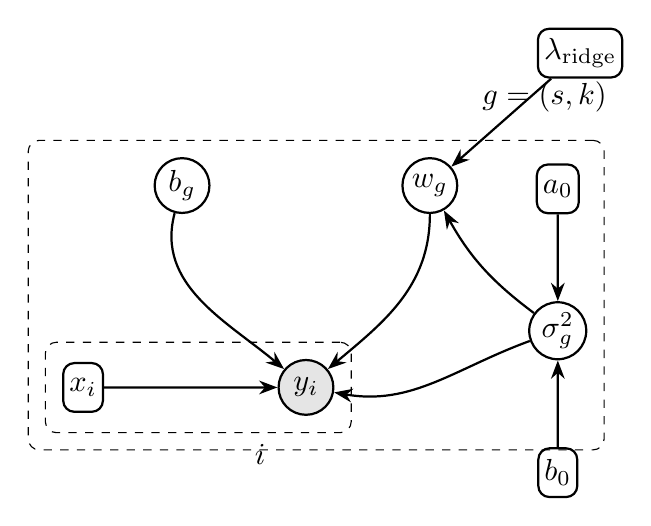
\begin{tikzpicture}[scale=1.1, transform shape]
  % Group-level parameters (independent per group).
  \node[rtlatent] (b) {$b_g$};
  \node[rtlatent, right=22mm of b] (w) {$w_g$};
  \node[rtlatent, below right=12mm and 10mm of w] (sig2) {$\sigma_g^2$};
  \node[rtconst, above right=10mm and 10mm of w] (lambda) {$\lambda_{\mathrm{ridge}}$};
  \node[rtconst, above=10mm of sig2] (a0) {$a_0$};
  \node[rtconst, below=10mm of sig2] (b0) {$b_0$};

  % Observations.
  \coordinate (bw_mid) at ($(b)!0.5!(w)$);
  \node[rtobs, below=20mm of bw_mid] (y) {$y_i$};
  \node[rtconst, left=20mm of y] (x) {$x_i$};

  % Edges (interpret ridge as a Gaussian prior / penalty on slopes).
  \path[rtarrow]
    (a0) edge (sig2)
    (b0) edge (sig2)
    (lambda) edge (w)
    (sig2) edge[bend left=12] (w)
    (b) edge[out=255, in=140] (y)
    (w) edge[out=270, in=40] (y)
    (sig2) edge[out=200, in=-10] (y)
    (x) edge (y);

  % Plates.
  \begin{scope}[on background layer]
    \node[rtplate, fit=(x) (y), label=below right:{$i$}] (plate_i) {};
    \node[rtplate, fit=(b) (w) (sig2) (plate_i), label={[yshift=2mm]above right:{$g=(s,k)$}}] {};
  \end{scope}
\end{tikzpicture}
\caption{Plate diagram for the sklearn supercategory ridge baseline. Each group $g=(s,k)$ (species\_cluster, comp\_id) is fit independently with ridge shrinkage on slopes $w_g$ (intercept $b_g$ unpenalized). The exported artifact stores a coefficient mean, an approximate coefficient covariance, and a per-group residual variance estimate $\sigma_g^2$ (from an inverse-gamma noise model with hyperparameters $a_0,b_0$).}
\label{fig:rt_sklearn_ridge_plate}
\end{figure}

\subsection{Baseline currently in production: supercategory lasso}
\label{subsec:rt_lasso_baseline}

The production baseline is a bank of lasso regressions fit per \texttt{(species\_cluster, comp\_id)} pair. Lasso is
attractive for sparse solutions, but its $\ell_1$ prior is a poor match to correlated run covariates and it does not
support partial pooling or chemistry-informed sharing across compounds. Its ``interval'' is a fixed window, not a
probabilistic prediction interval.

Each model stores point-estimate coefficients and a per-compound window scale derived from held-out residual variation.
At scoring time, Sally uses this to form an RT window half-width \codeword{expectedRTWindow} and then applies it as an RT
filter inside peak selection (described in the next subsection). Because this baseline does not expose a calibrated
predictive distribution, the window is best viewed as a heuristic tolerance rather than a nominal prediction interval.

\subsection{Baseline peak assignment in Sally: RT window filter + correction factor}
\label{subsec:sally_baseline_peak_selection}

Sally uses RT predictions in a deterministic per-task peak selection procedure. For a task $t$ and compound $c$, the RT
model provides an expected RT $\hat\mu_{t,c}$ and an RT window half-width $w_{t,c}$. A candidate peak with apex RT $r$
passes the RT filter when
\[
  \lvert r - \hat\mu_{t,c} \rvert \le w_{t,c}.
\]

For the production lasso baseline (\codeword{ESLASSO}), each compound model stores point-estimate coefficients and a base
window $w_{\mathrm{base},c}$ computed from held-out residuals as
\[
  w_{\mathrm{base},c} = 6\cdot \widehat{\mathrm{sd}}(\hat{y}-y),
\]
and the effective half-width used for filtering is scaled and clamped:
\[
  w_{t,c} = m\cdot \max(w_{\mathrm{base},c}, w_{\min}),
\]
with default $m=4$ and $w_{\min}=0.001$ minutes. For \codeword{COMPASSIGN_PP_RIDGE}, $w_{t,c}$ is derived from a
predictive distribution and varies by task (Section~\ref{eq:rt_pp_ridge_model} and the predictive-variance formula in the
inference section).

After RT filtering, some tasks can still contain multiple candidate peaks for the same compound. Sally resolves this by
computing an SSID-specific correction factor and then choosing the peak closest to the corrected center. For a retained
peak in task $t$ for compound $c$, define the signed residual
\[
  \Delta_{t,c} = \hat\mu_{t,c} - r.
\]
The correction factor is the median shift across tasks where the compound is observed:
\[
  \widehat{\mathrm{CF}}_c = \mathrm{median}_{t\in\mathcal{T}_c} \Delta_{t,c}.
\]
Within each task, Sally keeps the peak with smallest corrected distance $|\Delta_{t,c}-\widehat{\mathrm{CF}}_c|$ and
rejects the others. Finally, it removes outliers by keeping peaks within a fixed buffer
\[
  |\Delta_{t,c}-\widehat{\mathrm{CF}}_c| \le b,\qquad b=0.02 \text{ minutes}.
\]
The optional \codeword{iqr} method modifies only the centering step by restricting to a tighter ``central'' cloud when
computing $\widehat{\mathrm{CF}}_c$, but it applies the same fixed buffer after centering.

\begin{figure}[H]
\centering
\small
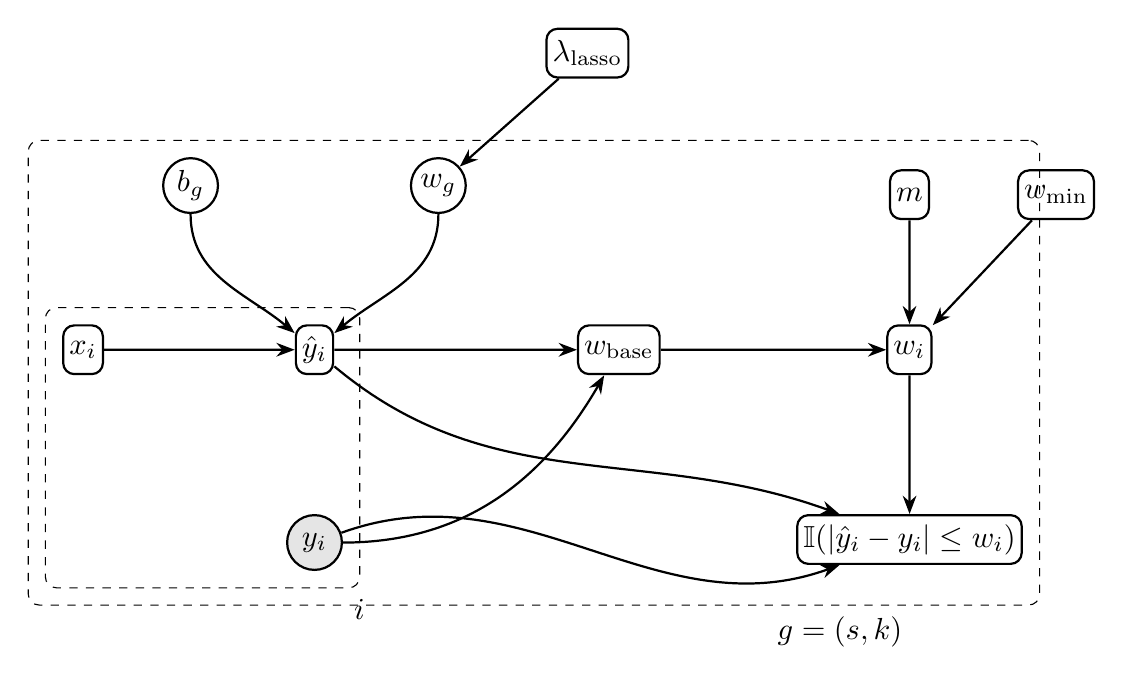
\begin{tikzpicture}[scale=1.1, transform shape]
  % Lasso point-estimate coefficients (independent per group).
  \node[rtlatent] (b) {$b_g$};
  \node[rtlatent, right=22mm of b] (w) {$w_g$};
  \node[rtconst, above right=10mm and 10mm of w] (alpha) {$\lambda_{\mathrm{lasso}}$};

  % Prediction + window heuristic.
  \coordinate (bw_mid) at ($(b)!0.5!(w)$);
  \node[rtconst, below=16mm of bw_mid] (yhat) {$\hat{y}_i$};
  \node[rtconst, left=22mm of yhat] (x) {$x_i$};
  \node[rtobs, below=16mm of yhat] (y) {$y_i$};

  \node[rtconst, right=28mm of yhat] (wbase) {$w_{\mathrm{base}}$};
  \node[rtconst, right=26mm of wbase] (wi) {$w_i$};
  \node[rtconst, below=16mm of wi] (keep) {$\mathbb{I}(|\hat{y}_i-y_i|\le w_i)$};

  \node[rtconst, above=12mm of wi] (m) {$m$};
  \node[rtconst, right=10mm of m] (wmin) {$w_{\min}$};

  % Edges.
  \path[rtarrow]
    (alpha) edge (w)
    (b) edge[out=270, in=140] (yhat)
    (w) edge[out=270, in=40] (yhat)
    (x) edge (yhat)
    (yhat) edge[out=0, in=180] (wbase)
    (y) edge[out=0, in=240] (wbase)
    (wbase) edge (wi)
    (m) edge (wi)
    (wmin) edge (wi)
    (wi) edge (keep)
    (yhat) edge[out=320, in=160] (keep)
    (y) edge[out=20, in=200] (keep);

  % Plates.
  \begin{scope}[on background layer]
    \node[rtplate, fit=(x) (yhat) (y), label=below right:{$i$}] (plate_i) {};
    \node[rtplate, fit=(b) (w) (plate_i) (wbase) (wi) (keep), label=below right:{$g=(s,k)$}] {};
  \end{scope}
\end{tikzpicture}
\caption{Schematic for the production supercategory lasso baseline (\codeword{ESLASSO}): each group $g=(s,k)$ (species\_cluster, comp\_id) stores point-estimate coefficients $(b_g,w_g)$ and a base window $w_{\mathrm{base}}$ from held-out residuals; scoring scales and clamps it to $w_i=m\max(w_{\mathrm{base}},w_{\min})$ and filters candidate peaks by the RT window.}
\label{fig:rt_lasso_plate}
\end{figure}

\subsection{RT coherence rejection via Bayesian Gaussian mixture}
\label{subsec:rt_coherence_mixture}
Sally's per-task selection is intentionally local: it applies a hard RT window filter, then picks the peak closest to the
(corrected) expected RT. This removes gross decoys, but some false positives still look plausible on individual tasks and
only become clearly inconsistent when aggregated across tasks for the same compound. We therefore add a
\emph{compound-level} coherence check for \codeword{COMPASSIGN_PP_RIDGE} that uses a continuous RT likelihood signal across
tasks.

The default setting is \codeword{peak_assignment_method} = \codeword{mixture_model}. Conceptually, it is a two-component Bayesian
Gaussian mixture model fitted \emph{within each SSID} to a single RT evidence score per compound.

The coherence rejection can be applied to any RT model that provides an expected mean and an RT window. In this report we
evaluate it with both \codeword{COMPASSIGN_PP_RIDGE} and \codeword{ESLASSO}. For \codeword{ESLASSO}, the score should be
interpreted as a pseudo-likelihood because the window is heuristic rather than a calibrated predictive sd.

\begin{figure}[H]
\centering
\includegraphics[width=0.95\linewidth]{mixture_model_example_ssid12307_lib208.png}
\caption{Example \codeword{mixture_model} coherence check for SSID 12307 (lib208).
Left: histogram of per-compound scores $x_c$ with the fitted two-component mixture and the
$p(\mathrm{coherent}\mid x_c)=0.5$ decision boundary.
Right: per-task normalized residuals $z_{t,c}$ for an example \emph{kept} compound and an example \emph{rejected}
compound, illustrating coherent vs.\ incoherent across-task behavior.}
\label{fig:mixture_model_example_12307}
\end{figure}

\begin{enumerate}
  \item \emph{Per-peak RT log-likelihood.} After selecting a peak for compound $c$ in task $t$, let $r_{t,c}$ be the
  observed apex RT and let the RT model provide an expected mean $\hat\mu_{t,c}$ and window half-width $w_{t,c}$.
  We convert the half-width to an sd-like scale using the nominal 95\% relationship
  $\sigma_{t,c} = w_{t,c}/z_{0.975}$ (after applying any global window multiplier). We also apply Sally's per-compound
  correction factor $\widehat{\mathrm{CF}}_{c}$ (median RT shift across tasks within the SSID). Define the signed residual
  $\Delta_{t,c}=\hat\mu_{t,c}-r_{t,c}$ and the standardized residual and RT log-likelihood score as
  \[
    z_{t,c} = \frac{\Delta_{t,c}-\widehat{\mathrm{CF}}_{c}}{\sigma_{t,c}},
    \qquad
    \ell_{t,c} = \log p(r_{t,c}\mid \hat\mu_{t,c},\sigma_{t,c})
    = -\tfrac{1}{2}\Bigl(z_{t,c}^2+\log \sigma_{t,c}^2\Bigr),
  \]
  where $\ell_{t,c}$ is the Normal log predictive density up to an additive constant. In code this is computed as an
  internal feature (stored as \texttt{\_rt\_loglik} during the mixture fit).

  \item \emph{One scalar score per compound.} For each compound $c$ in an SSID, we aggregate over LC tasks with a selected
  peak and define
  \[
    x_c = \frac{1}{n_c}\sum_{t\in \mathcal{T}_c} \ell_{t,c},
  \]
  where $\mathcal{T}_c$ is the set of contributing tasks and $n_c=|\mathcal{T}_c|$.
  This compresses the across-task RT evidence for a compound into a single scalar that can be modeled across compounds.

  \item \emph{Two-component Gaussian mixture within an SSID.} Within a fixed SSID, we model the set of compound scores
  $\{x_c\}$ as coming from a mixture of two Gaussian populations:
  \[
    z_c \sim \mathrm{Categorical}(\pi),
    \qquad
    x_c\mid z_c=k \sim \mathcal{N}(\mu_k,\sigma_k^2),
    \qquad k\in\{1,2\}.
  \]
  The mixture is over compounds within the SSID: each observation is a compound-level summary statistic $x_c$ (already
  aggregated across tasks). We use conjugate priors
  \[
    \pi \sim \mathrm{Dirichlet}(\alpha_0,\alpha_0),
    \qquad
    \tau_k \equiv \sigma_k^{-2} \sim \mathrm{Gamma}(a_0,b_0),
    \qquad
    \mu_k\mid \tau_k \sim \mathcal{N}\!\left(m_0,\;(\kappa_0\tau_k)^{-1}\right),
  \]
  which is the 1D Normal--Gamma form of the Normal--Wishart prior used by variational Bayesian Gaussian mixture models. In
  code we set $\alpha_0=0.5$ (encourages, but does not force, an imbalanced mixture) and use a small covariance
  regularizer; remaining hyperparameters follow the library defaults.

  \item \emph{Inference outputs.} We infer an approximate posterior over component parameters and compound memberships. In
  particular, variational Bayes produces responsibilities
  \[
    r_{c,k} \equiv p(z_c=k\mid x_c),
    \qquad \sum_k r_{c,k}=1,
  \]
  along with posterior summaries for $\pi$, $\mu_k$, and $\sigma_k^2$.
  Implementation uses scikit-learn's variational Bayesian Gaussian mixture implementation.

  \item \emph{Identifying the coherent component.} The fitted mixture produces two clusters with weights $\pi_k$ and means
  $\mu_k$. After the per-task RT window filter, most compounds are expected to be coherent, so we label the coherent
  cluster as the one with the larger fitted weight:
  \[
    k^\star = \arg\max_k \pi_k.
  \]
  The corresponding mean $\mu_{k^\star}$ summarizes typical coherent RT evidence in that SSID, while the other component
  captures a lower-likelihood population. Together $(\pi_k,\mu_k,\sigma_k^2)$ define an implicit, data-driven boundary for
  ``coherent enough'' without a fixed global threshold.

  \item \emph{Rejection rule.} For each compound we compute its posterior coherence probability
  $p_c = r_{c,k^\star}$. If $p_c<0.5$ we reject the compound (MAP under equal misclassification costs) by removing all of
  its selected peaks from \texttt{bundle.peaks}; the standard Sally pipeline then marks the compound \texttt{IGNORE}.
\end{enumerate}

The score $x_c$ is a \emph{likelihood} under a Normal model whose scale $\sigma_{t,c}$ is derived directly from the RT
window $w_{t,c}$. For \codeword{COMPASSIGN_PP_RIDGE}, $w_{t,c}$ is computed from a probabilistic predictive variance and
varies by task (2D window matrix), so $z_{t,c}$ and $\ell_{t,c}$ behave like a calibrated standardized residual and log
predictive density. This makes $x_c$ a meaningful continuous coherence signal.
For \codeword{ESLASSO}, the RT window is a per-compound heuristic (1D; constant across tasks) rather than an inferred
predictive sd, so after centering by $\widehat{\mathrm{CF}}_c$ the compound score $x_c$ is dominated by the window term
$-\tfrac{1}{2}\log \sigma_{t,c}^2$ rather than residual coherence (in our runs, $\mathrm{corr}(x_c,\overline{\log\sigma^2})
\approx -1$). The resulting mixture primarily separates compounds by their heuristic window width, which can reject many
true compounds and reduce recall.

\section{Evaluation}

We compare models trained on the capped \texttt{cap100} dataset and evaluated on the held-out test split for lib208 and
lib209. This report focuses on the standard seen-compound evaluation where models score nearly all rows and the
comparison is driven by accuracy and calibrated windows rather than missing-model fallbacks. To focus on \emph{model form}
rather than feature engineering, we use the same linear run covariates for all models (no polynomial expansions).

\subsection{Data preparation}
All offline training and evaluation inputs are built by \path{src/compassign/rt/prep.sh}. Starting from Pachyderm, it
produces merged Parquets under \path{repo_export/merged_training/} and then derives the training caps and evaluation CSVs
used throughout this report. In outline, the pipeline is:
\begin{itemize}
  \item \emph{Fetch training shards from Pachyderm.} Use \codeword{pachctl get file} to download
  \codeword{create_training_data} and \codeword{combine_predictors} outputs for each library from fixed job IDs (project
  \codeword{autocuration_platinum}) into \path{repo_export/pachyderm_rt_training_raw/}.
  \item \emph{Assemble a combined export tree.} Copy the per-library shard trees into a stable layout under
  \path{repo_export/pachyderm_rt_training_latest/}.
  \item \emph{Merge shards into a single Parquet.} Run
  \path{src/compassign/rt/data_prep/merge_pachyderm_training.py} to create
  \path{repo_export/merged_training/merged_training_all.parquet}.
  \item \emph{Split by library.} Run \path{src/compassign/rt/data_prep/split_merged_by_lib.py} to produce per-library
  Parquets under \path{repo_export/merged_training/}.
  \item \emph{Regenerate strict species mappings.} Run
  \path{src/compassign/rt/data_prep/check_rt_metadata_mapping.py} to ensure a consistent mapping from \texttt{sample\_set\_id}
  to \texttt{species} and \texttt{species\_cluster}.
  \item \emph{Build capped training datasets (\texttt{cap100}).} For each (supercategory, species, compound) group, keep at
  most 100 rows using uniform random sampling with a fixed seed (42) via
  \path{src/compassign/rt/data_prep/build_rt_cap_datasets.sh} (which calls
  \path{src/compassign/rt/data_prep/sample_per_species_compound.py}). These capped CSVs are the training inputs for all
  reported models.
  \item \emph{Build held-out test CSVs (evaluation input).} Filter the merged Parquet to SSIDs assigned to the \texttt{test}
  fold in \path{data/split_outputs/train_test_split_all.csv} and convert each SSID to RT production-style CSVs via
  \path{src/compassign/rt/data_prep/build_rt_real_test_csvs.py}.
\end{itemize}

\subsection{Metrics}
Let $y_i$ be observed RT and $\hat{y}_i$ the point prediction (minutes).
\begin{itemize}
  \item RMSE: $\sqrt{\frac{1}{n}\sum_i (\hat{y}_i - y_i)^2}$.
  \item MAE: $\frac{1}{n}\sum_i |\hat{y}_i - y_i|$.
  \item Cov95 (ridge models): define predicted variance as
  \[
  \begin{aligned}
    \widehat{\mathrm{Var}}(y_i\mid x_{i,1:p})
    &\approx \sigma^2_{g(i)} \\
    &\quad + \sum_{a=0}^{p}\sum_{b=0}^{p}
      \tilde{x}_{i,a}\tilde{x}_{i,b}\,
      \widehat{\mathrm{Cov}}\!\left(\beta_{g(i),a},\beta_{g(i),b}\right),
  \end{aligned}
  \]
  with predicted standard deviation $\hat{\sigma}_i=\sqrt{\widehat{\mathrm{Var}}(y_i\mid x_{i,1:p})}$ and
  $k_{0.95}=\Phi^{-1}(0.975)\approx 1.96$.
  We define the nominal 95\% interval as $\hat{y}_i \pm k_{0.95}\,\hat{\sigma}_i$ and count row $i$ as ``covered'' if
  $|\hat{y}_i - y_i| \le k_{0.95}\,\hat{\sigma}_i$; Cov95 is the empirical fraction of covered rows.
  The terms $\sigma^2_{g(i)}$ and $\widehat{\mathrm{Cov}}(\beta_{g(i)})$ come from the exported stage-1 coefficient summaries:
  for the sklearn ridge baseline they are computed analytically from ridge normal equations with an inverse-gamma noise prior,
  while for the partial pooling model they are computed in closed form conditional on fitted hierarchical hyperparameters
  (an empirical-Bayes plug-in approximation).
  \item Width95 (ridge models): $\frac{1}{n}\sum_i 2\cdot k_{0.95}\cdot \hat{\sigma}_i$.
\end{itemize}

In the expressions above, $g(i)$ denotes the coefficient-summary group for row $i$, and we use the augmented covariates
$\tilde{x}_{i,0}=1$ and $\tilde{x}_{i,j}=x_{i,j}$ for $j=1,\ldots,p$.
For the production lasso baseline, the ``window'' is a fixed filtering half-width derived from held-out residuals and then
scaled by a global multiplier (see Section~\ref{subsec:rt_lasso_baseline}). This window is not calibrated to a nominal
95\% target, so we do not report it as Cov95/Width95.

\section{Results: offline RT regression}

\subsection{Global performance}

Table~\ref{tab:global_metrics} summarizes global metrics on the held-out test split for lib208 and lib209. Lasso baselines do not
score all rows; the Rows scored column reflects applicability.

\begin{table}[H]
\centering
\caption{Global held-out test metrics for cap100-trained models (linear features). Cov95/Width95 report empirical coverage and
mean width of the nominal 95\% Normal interval $\hat{y}_i \pm k_{0.95}\,\hat{\sigma}_i$ and are only defined for ridge
models with an explicit predictive variance. The lasso baseline uses a heuristic fixed filtering window; its Cov95/Width95
entries are omitted (--) to avoid implying nominal calibration.}
\label{tab:global_metrics}
\begin{tabular}{llrrrrrr}
\toprule
Lib & Model & RMSE & MAE & Cov95 & Width95 & Rows scored & Train (min) \\
\midrule
208 & Ridge (supercategory) & 0.009050 & 0.004684 & 0.944 & \textbf{0.023573} & \textbf{100.0\%} & \textbf{0.0} \\
208 & Ridge (partial pooling) & \textbf{0.007846} & \textbf{0.003817} & \textbf{0.958} & 0.028744 & \textbf{100.0\%} & 131.0 \\
208 & Lasso (supercategory) & 0.015081 & 0.007956 & -- & -- & 94.7\% & -- \\
\midrule
209 & Ridge (supercategory) & 0.008295 & 0.004631 & 0.919 & \textbf{0.020994} & \textbf{100.0\%} & \textbf{0.0} \\
209 & Ridge (partial pooling) & \textbf{0.007589} & \textbf{0.004203} & \textbf{0.957} & 0.027094 & \textbf{100.0\%} & 242.3 \\
209 & Lasso (supercategory) & 0.009439 & 0.004954 & -- & -- & 97.8\% & -- \\
\bottomrule
\end{tabular}
\end{table}

Relative to Ridge (supercategory), Ridge (partial pooling) improves RMSE while moving coverage
closer to the nominal 0.95 target. This is desirable for peak assignment because under-coverage translates directly into
missed true peaks when the window is used as a hard filter.
The lasso baseline is included for context: it does not score all rows and its uncertainty is a fixed window rather than
a probabilistic interval.

\begin{figure}[H]
\centering
\includegraphics[width=0.95\linewidth]{lib208_global_comparison_anchor_none_full.png}
\caption{Global comparison across report baselines for lib208 (cap100 training, held-out test evaluation). Panels show RMSE,
Cov95 (ridge models only; lasso omitted), and mean RT window width (Width95 for ridge models; production filtering window
for lasso). Tighter windows are only meaningful when coverage is comparable.}
\label{fig:global_comparison_lib208}
\end{figure}

\begin{figure}[H]
\centering
\includegraphics[width=0.95\linewidth]{lib209_global_comparison_anchor_none_full.png}
\caption{Global comparison across report baselines for lib209 (cap100 training, held-out test evaluation). Panels show RMSE,
Cov95 (ridge models only; lasso omitted), and mean RT window width (Width95 for ridge models; production filtering window
for lasso). Tighter windows are only meaningful when coverage is comparable.}
\label{fig:global_comparison_lib209}
\end{figure}

\subsection{Interval calibration: supercategory ridge vs partial pooling}

The sklearn ridge baseline and the proposed hierarchical ridge model are both linear in the same run covariates, but
they differ in how information is shared across sparse groups and in how predictive variance is formed. Empirically, the
sklearn baseline produces narrower windows but under-covers the nominal 95\% target (coverage $\sim$0.92--0.94). The
hierarchical model yields coverage closer to nominal at moderately larger width.

\subsection{Performance by species\_cluster}

Figures~\ref{fig:by_cluster_lib208} and \ref{fig:by_cluster_lib209} aggregate metrics by \texttt{species\_cluster}.

\begin{figure}[H]
\centering
\includegraphics[width=0.95\linewidth]{lib208_by_species_cluster_anchor_none_full.png}
\caption{Metrics by \texttt{species\_cluster} (supercategory) for lib208 report baselines. The Cov95 panel excludes lasso
because its fixed filtering window is not a nominal probabilistic interval; mean RT window width includes the lasso
filtering window for context.}
\label{fig:by_cluster_lib208}
\end{figure}

\begin{figure}[H]
\centering
\includegraphics[width=0.95\linewidth]{lib209_by_species_cluster_anchor_none_full.png}
\caption{Metrics by \texttt{species\_cluster} (supercategory) for lib209 report baselines. The Cov95 panel excludes lasso
because its fixed filtering window is not a nominal probabilistic interval; mean RT window width includes the lasso
filtering window for context.}
\label{fig:by_cluster_lib209}
\end{figure}

\section{Results: end-to-end Sally evaluation}
\subsection{Setup}

Offline split evaluation is necessary but not sufficient for deployment: in production, the RT model is used inside
Sally's peak assignment pipeline as a hard filter and interacts with other stages (candidate generation, peak selection,
and post-processing). We therefore evaluate end-to-end peak assignment using \texttt{sally-dev evaluate}.
We compare the current production baseline RT model bundle (supercategory lasso; \codeword{ESLASSO}) against the proposed
CompAssign partial pooling ridge bundle exported as stage-1 coefficient summaries (\codeword{COMPASSIGN_PP_RIDGE}). We
report precision/recall/Threat Score (TS) from Sally's \texttt{mdsutils} summary.

We also compare two peak-selection modes: Sally's standard within-task selection logic
(\codeword{peak_assignment_method}=\codeword{baseline}) and the compound-level RT coherence rejection described in
Section~\ref{subsec:rt_coherence_mixture} (\codeword{peak_assignment_method}=\codeword{mixture_model}). This yields a
$2{\times}2$ ablation over (i) RT model (\codeword{ESLASSO} vs \codeword{COMPASSIGN_PP_RIDGE}) and (ii) peak assignment
method (\codeword{baseline} vs \codeword{mixture_model}). In these runs, \codeword{COMPASSIGN_PP_RIDGE} uses a widened RT
window multiplier ($m=4$).

We evaluated eight held-out cell-type SSIDs from supercategories 6 and 8 (two SSIDs per supercategory per library),
selected from the test fold of \path{data/split_outputs/train_test_split_all.csv}. For lib208:
SSID 12307 and SSID 12725 (supercat 6), and SSID 12609 and SSID 13208 (supercat 8).
For lib209: SSID 23059 and SSID 23146 (supercat 6), and SSID 20159 and SSID 20814
(supercat 8).
For reproducibility, \nolinkurl{src/compassign/rt/sally_test.sh} re-runs the exact SSIDs and extracts metrics from the
\texttt{mdsutils} summary pickles. Sally integration details are listed in Appendix~\ref{app:sally_integration}.

\subsection{Results}
Tables~\ref{tab:sally_prelim_cells_lib208} and \ref{tab:sally_prelim_cells_lib209} report the end-to-end peak-assignment
metrics from Sally's \texttt{mdsutils} summary pickles. Higher is better for all three metrics. For each SSID, the
baseline and \codeword{COMPASSIGN_PP_RIDGE} were run with the same evaluation mode (\texttt{mdsutils}).

\begin{table}[H]
\centering
\caption{Preliminary end-to-end Sally evaluation on selected cell-type SSIDs (lib208; supercategories 6 and 8). Metrics
are precision, recall, and Threat Score (TS) from \texttt{mdsutils}. Bold indicates the best value within each SSID.}
\label{tab:sally_prelim_cells_lib208}
\begin{tabular}{lllrrr}
\toprule
Supercat & SSID & Setting & Precision & Recall & TS \\
\midrule
6 & 12307 & \codeword{ESLASSO} + \codeword{baseline} & 0.8436 & 0.7848 & 0.6851 \\
6 & 12307 & \codeword{ESLASSO} + \codeword{mixture_model} & 0.8300 & 0.4737 & 0.4318 \\
6 & 12307 & \codeword{COMPASSIGN_PP_RIDGE} + \codeword{baseline} & 0.9390 & 0.8113 & 0.7706 \\
6 & 12307 & \codeword{COMPASSIGN_PP_RIDGE} + \codeword{mixture_model} & \textbf{0.9480} & \textbf{0.8122} & \textbf{0.7776} \\
\midrule
6 & 12725 & \codeword{ESLASSO} + \codeword{baseline} & 0.6808 & 0.8610 & 0.6134 \\
6 & 12725 & \codeword{ESLASSO} + \codeword{mixture_model} & 0.6808 & 0.8610 & 0.6134 \\
6 & 12725 & \codeword{COMPASSIGN_PP_RIDGE} + \codeword{baseline} & 0.8285 & \textbf{0.8810} & 0.7451 \\
6 & 12725 & \codeword{COMPASSIGN_PP_RIDGE} + \codeword{mixture_model} & \textbf{0.9303} & \textbf{0.8810} & \textbf{0.8264} \\
\midrule
8 & 12609 & \codeword{ESLASSO} + \codeword{baseline} & 0.8553 & 0.6513 & 0.5867 \\
8 & 12609 & \codeword{ESLASSO} + \codeword{mixture_model} & 0.8593 & 0.5410 & 0.4970 \\
8 & 12609 & \codeword{COMPASSIGN_PP_RIDGE} + \codeword{baseline} & 0.8417 & 0.8070 & 0.7006 \\
8 & 12609 & \codeword{COMPASSIGN_PP_RIDGE} + \codeword{mixture_model} & \textbf{0.9320} & \textbf{0.8073} & \textbf{0.7624} \\
\midrule
8 & 13208 & \codeword{ESLASSO} + \codeword{baseline} & 0.8931 & 0.7930 & 0.7243 \\
8 & 13208 & \codeword{ESLASSO} + \codeword{mixture_model} & 0.8931 & 0.7930 & 0.7243 \\
8 & 13208 & \codeword{COMPASSIGN_PP_RIDGE} + \codeword{baseline} & 0.8546 & 0.7930 & 0.6987 \\
8 & 13208 & \codeword{COMPASSIGN_PP_RIDGE} + \codeword{mixture_model} & \textbf{0.9555} & \textbf{0.7973} & \textbf{0.7688} \\
\bottomrule
\end{tabular}
\end{table}

\begin{table}[H]
\centering
\caption{Preliminary end-to-end Sally evaluation on selected cell-type SSIDs (lib209; supercategories 6 and 8). Metrics
are precision, recall, and Threat Score (TS) from \texttt{mdsutils}. Bold indicates the best value within each SSID.}
\label{tab:sally_prelim_cells_lib209}
\begin{tabular}{lllrrr}
\toprule
Supercat & SSID & Setting & Precision & Recall & TS \\
\midrule
6 & 23059 & \codeword{ESLASSO} + \codeword{baseline} & 0.8357 & 0.5940 & 0.5319 \\
6 & 23059 & \codeword{ESLASSO} + \codeword{mixture_model} & 0.8357 & 0.5940 & 0.5319 \\
6 & 23059 & \codeword{COMPASSIGN_PP_RIDGE} + \codeword{baseline} & 0.8164 & \textbf{0.6868} & 0.5949 \\
6 & 23059 & \codeword{COMPASSIGN_PP_RIDGE} + \codeword{mixture_model} & \textbf{0.8913} & 0.6852 & \textbf{0.6324} \\
\midrule
6 & 23146 & \codeword{ESLASSO} + \codeword{baseline} & 0.6732 & 0.8257 & 0.5894 \\
6 & 23146 & \codeword{ESLASSO} + \codeword{mixture_model} & 0.6732 & 0.8257 & 0.5894 \\
6 & 23146 & \codeword{COMPASSIGN_PP_RIDGE} + \codeword{baseline} & 0.6800 & 0.8686 & 0.6166 \\
6 & 23146 & \codeword{COMPASSIGN_PP_RIDGE} + \codeword{mixture_model} & \textbf{0.9857} & \textbf{0.8692} & \textbf{0.8584} \\
\midrule
8 & 20159 & \codeword{ESLASSO} + \codeword{baseline} & 0.8865 & 0.8697 & 0.7825 \\
8 & 20159 & \codeword{ESLASSO} + \codeword{mixture_model} & 0.8865 & 0.8697 & 0.7825 \\
8 & 20159 & \codeword{COMPASSIGN_PP_RIDGE} + \codeword{baseline} & 0.8906 & \textbf{0.8848} & 0.7980 \\
8 & 20159 & \codeword{COMPASSIGN_PP_RIDGE} + \codeword{mixture_model} & \textbf{0.9871} & \textbf{0.8848} & \textbf{0.8747} \\
\midrule
8 & 20814 & \codeword{ESLASSO} + \codeword{baseline} & 0.9123 & 0.8695 & 0.8024 \\
8 & 20814 & \codeword{ESLASSO} + \codeword{mixture_model} & 0.9123 & 0.8695 & 0.8024 \\
8 & 20814 & \codeword{COMPASSIGN_PP_RIDGE} + \codeword{baseline} & 0.9194 & \textbf{0.8783} & 0.8155 \\
8 & 20814 & \codeword{COMPASSIGN_PP_RIDGE} + \codeword{mixture_model} & \textbf{0.9687} & 0.8753 & \textbf{0.8513} \\
\bottomrule
\end{tabular}
\end{table}

Across these eight SSIDs, the strongest setting is consistently the combination of \codeword{COMPASSIGN_PP_RIDGE} with
\codeword{mixture_model}, which improves TS relative to the production \codeword{ESLASSO} baseline for all eight checks.
Within \codeword{COMPASSIGN_PP_RIDGE}, \codeword{mixture_model} improves TS versus \codeword{baseline} in every case.
In contrast, applying \codeword{mixture_model} to \codeword{ESLASSO} does not help and can substantially reduce recall/TS
(e.g.\ SSIDs 12307 and 12609 in Table~\ref{tab:sally_prelim_cells_lib208}).

\subsection{Notes}
The \texttt{mdsutils} TS in Tables~\ref{tab:sally_prelim_cells_lib208} and \ref{tab:sally_prelim_cells_lib209} includes
false negatives for curated internal standards and X-compounds, which are omitted from production outputs by design.
We therefore treat these TS values as conservative when judging production impact, and interpret TS deltas in the context
of the ``do not call standards / X-compounds'' constraint.

For these cap100-trained lib208/lib209 models, the coefficient-summary artifacts include compounds with missing chemistry
metadata (missing \texttt{chemical\_id} or missing ChemBERTa embeddings). For lib208, the trainer uses mean-embedding
fallback for 310 compounds with missing \texttt{chemical\_id} and 138 compounds with missing embeddings; for lib209, this is
990 and 540 compounds, respectively. This prevents coverage holes in the Sally integration (avoids ``No RT model'') at the
cost of disabling the chemistry-informed prior mean for those compounds (chemistry term uses $z_c=0$).

\section{Discussion and conclusion}

\subsection{Summary of findings}
Offline split evaluation shows that \codeword{COMPASSIGN_PP_RIDGE} improves RT prediction and produces RT windows with
coverage close to the nominal 95\% target. This matters because Sally uses RT windows as a hard filter: if the window is
too narrow, true peaks are removed (false negatives); if it is too wide, decoys survive and can become false positives.
Relative to the fast supercategory ridge baseline, the hierarchical model improves RMSE while reducing under-coverage.

End-to-end evaluation inside Sally confirms these improvements translate to peak assignment performance when combined with
the across-task coherence check. On eight held-out SSIDs (Tables~\ref{tab:sally_prelim_cells_lib208} and
\ref{tab:sally_prelim_cells_lib209}), \codeword{COMPASSIGN_PP_RIDGE} with \codeword{mixture_model} improves Threat Score
(TS) versus the current \codeword{ESLASSO} baseline on all checks (lib208: approximately +0.04 to +0.21; lib209:
approximately +0.05 to +0.27). Within \codeword{COMPASSIGN_PP_RIDGE}, the coherence check improves TS versus the baseline
within-task peak picker for every SSID evaluated. This supports the central hypothesis: RT evidence is often strongest
when aggregated across tasks, and a compound-level coherence score can remove false positives that survive per-task
filtering.

\subsection{Why the coherence score works}
The mixture-based coherence check is most reliable when the underlying RT model produces a calibrated predictive sd. For
\codeword{COMPASSIGN_PP_RIDGE}, the per-task window is derived from an explicit predictive variance, so the per-task RT
log-likelihood behaves like a standardized residual score. This makes the compound score $x_c$ a meaningful continuous
signal and allows the mixture model to adapt its separation boundary to each SSID.

By contrast, for \codeword{ESLASSO} the window is heuristic and constant across tasks, so the same score behaves like a
pseudo-likelihood and can be dominated by window width rather than true coherence. In practice this can lead to
over-rejection and recall loss on some SSIDs. This difference highlights a key practical point: if RT uncertainty is used
downstream as a hard filter and as a likelihood scale, then having a probabilistic RT model is not just ``nicer''---it can
change the behavior of compound-level aggregation in a qualitatively important way.

\subsection{Limitations and future work}
The main practical downside of the hierarchical model is training cost: variational inference over the hierarchy is far
slower than independent ridge fits. This makes the hierarchical model best suited to offline retrains (periodic model
refreshes), while the fast sklearn ridge baseline remains useful for quick iteration and regression checks. The lasso
baseline remains valuable as a historical point of comparison, but its lack of hierarchy and its heuristic uncertainty
windows make it a weaker fit for modern peak assignment requirements.

The end-to-end evaluation in this report is intentionally scoped: it covers a small set of SSIDs and focuses on
single-library checks. Before deployment, the most important next step is to expand evaluation across more SSIDs
(including multi-library sample sets) and to confirm that RT window calibration remains stable under different run
conditions and post-processing settings. Separately, the \codeword{mixture_model} coherence probability could be exposed
as a soft confidence score (instead of a hard rejection) to support explicit precision/recall trade-offs in downstream
reporting.

\subsection{Unseen species (exploratory holdouts)}

The main results focus on seen-compound performance. To probe cold-start for new species, we ran exploratory group
holdouts on a production subset with two modes:
\begin{itemize}
  \item \texttt{species}: hold out entire species within each \texttt{species\_cluster},
  \item \texttt{species\_comp}: hold out (\texttt{species}, \texttt{comp\_id}) pairs. For each held-out pair, we keep the
  corresponding \texttt{species\_cluster} and \texttt{comp\_id} observed in training.
\end{itemize}

We evaluate the hierarchical ridge model with an explicit unseen-species backoff (aggregate fitted
(\texttt{species}, \texttt{comp\_id}) coefficients across training species to form a supercategory--compound coefficient), compare
to the supercategory ridge baseline, and include the legacy lasso bundle for context.

\begin{table}[H]
\centering
\caption{Unseen holdout metrics (lib208 production subset; seed=42; holdout\_frac=0.2; clusters=4,5; top\_comp\_ids=100).}
\label{tab:unseen_holdout_lib208}
\begin{tabular}{llrrrrr}
\toprule
Holdout & Model & RMSE & MAE & Cov95 & Rows scored (\%) \\
\midrule
\texttt{species} & Ridge (partial pooling) & 0.014968 & 0.009012 & 1.000 & \textbf{100.0} \\
\texttt{species} & Ridge (supercategory) & 0.011090 & 0.005202 & 0.877 & \textbf{100.0} \\
\texttt{species} & Lasso (supercategory, external) & \textbf{0.007913} & \textbf{0.004174} & -- & 94.8 \\
\midrule
\texttt{species\_comp} & Ridge (partial pooling) & 0.013474 & 0.009569 & 1.000 & \textbf{100.0} \\
\texttt{species\_comp} & Ridge (supercategory) & 0.013272 & 0.006532 & 0.812 & \textbf{100.0} \\
\texttt{species\_comp} & Lasso (supercategory, external) & \textbf{0.007671} & \textbf{0.004331} & -- & 94.9 \\
\bottomrule
\end{tabular}
\end{table}

\begin{table}[H]
\centering
\caption{Unseen holdout metrics (lib209 production subset; seed=42; holdout\_frac=0.2; clusters=4,5; top\_comp\_ids=100).}
\label{tab:unseen_holdout_lib209}
\begin{tabular}{llrrrrr}
\toprule
Holdout & Model & RMSE & MAE & Cov95 & Rows scored (\%) \\
\midrule
\texttt{species} & Ridge (partial pooling) & 0.008381 & 0.005281 & 1.000 & \textbf{100.0} \\
\texttt{species} & Ridge (supercategory) & 0.008268 & 0.004870 & 0.902 & \textbf{100.0} \\
\texttt{species} & Lasso (supercategory, external) & \textbf{0.006779} & \textbf{0.004267} & -- & 92.4 \\
\midrule
\texttt{species\_comp} & Ridge (partial pooling) & 0.011684 & 0.006456 & 1.000 & \textbf{100.0} \\
\texttt{species\_comp} & Ridge (supercategory) & 0.013582 & 0.006320 & 0.883 & \textbf{100.0} \\
\texttt{species\_comp} & Lasso (supercategory, external) & \textbf{0.009482} & \textbf{0.005677} & -- & 95.0 \\
\bottomrule
\end{tabular}
\end{table}

These holdouts suggest that an explicit backoff strategy can make the hierarchical model usable for unseen species as
long as the supercategory remains known. The high coverage values indicate the backoff is conservative; improving
precision under unseen species will likely require either a stronger species hierarchy (so truly unseen species can be
handled without ad-hoc aggregation) or small amounts of new-species calibration data.

\subsection{Unseen compounds (zero-shot chemistry)}

To isolate true compound cold-start, we ran a held-out chemistry experiment where \texttt{chem\_id} values are removed
entirely from training. We compare the hierarchical ridge model (which can still score via the chemistry prior mean) to a
non-linear single-model embedding baseline (MLP) that uses ChemBERTa PCA-20 features for point prediction.

\begin{table}[H]
\centering
\caption{Zero-shot chemistry results on the lib208 production subset (hold out 20 \texttt{chem\_id}; seed=42).}
\label{tab:zero_shot_lib208}
\begin{tabular}{lrrr}
\toprule
Model & RMSE & MAE & Cov95 \\
\midrule
Ridge (partial pooling) & 1.049358 & 0.699639 & \textbf{1.000} \\
MLP (ChemBERTa PCA-20 + cluster interactions) & \textbf{0.468125} & \textbf{0.345321} & -- \\
\bottomrule
\end{tabular}
\end{table}

\begin{table}[H]
\centering
\caption{Zero-shot chemistry results on the lib209 production subset (hold out 20 \texttt{chem\_id}; seed=42).}
\label{tab:zero_shot_lib209}
\begin{tabular}{lrrr}
\toprule
Model & RMSE & MAE & Cov95 \\
\midrule
Ridge (partial pooling) & 1.523705 & 1.062139 & \textbf{0.991} \\
MLP (ChemBERTa PCA-20 + cluster interactions) & \textbf{1.061293} & \textbf{0.799969} & -- \\
\bottomrule
\end{tabular}
\end{table}

Point accuracy in the true zero-shot setting is currently much better for the non-linear embedding baseline, which
suggests the linear chemistry head inside the hierarchical model is not yet expressive enough. However, the hierarchical
model still provides a calibrated uncertainty estimate, which is valuable for windowing. Improving the chemistry head
while keeping the residual per-compound term $\delta_k$ (so seen-compound performance is maintained) is the key next step.

Two practical extensions are: (i) add a compound-class anchor term so unseen compounds can back off to a learned class
mean when embeddings are weak, and (ii) increase shrinkage on the chemistry-head coefficients $\theta_{\alpha,1:D}$
(or use global shrinkage priors) to
avoid high-variance extrapolation on held-out chemistries.

In conclusion, the combination of a probabilistic RT regression model and an SSID-specific coherence score provides a
more principled RT pipeline for autocuration: calibrated per-task uncertainty supports reliable RT filtering, and the
mixture-based compound-level probability provides a continuous, data-adaptive criterion for rejecting likely false
positives without a fixed global threshold. The remaining work is to broaden end-to-end evaluation and to improve
cold-start behavior for truly unseen species and chemistries while preserving seen-compound performance.

\appendix

\section{Sally integration details}
\label{app:sally_integration}

To support \codeword{COMPASSIGN_PP_RIDGE} end-to-end inside \texttt{sally-dev}, we made the following focused changes:
\begin{itemize}
  \item Added \codeword{modelType=COMPASSIGN_PP_RIDGE} which loads CompAssign stage-1 coefficient summaries and backoff
  summaries (both shipped as \texttt{.npz} artifacts), and computes per-task RT windows from predictive variance.
  \item Generalized Sally's regression predictor so RT windows can be either per-compound (1D) or per-(task,compound) (2D),
  since \codeword{COMPASSIGN_PP_RIDGE} produces row-specific uncertainty.
  \item Added CompAssign RT inputs (species, species\_cluster, and covariates CSV) and \texttt{--force-curate} to run the
  full curation pipeline for evaluation even when a sample set would normally be skipped.
  \item Updated \texttt{sally-dev evaluate} to fail fast when the underlying pipeline run fails (instead of continuing with
  stale cached pickles), and updated the pipeline wrapper and \codeword{COMPASSIGN_PP_RIDGE} loader so production-style RT
  covariates can be mounted into the Docker container and read efficiently by streaming only the required task IDs
  (important for multi-GB lib209 covariates CSVs).
\end{itemize}

\section{Collapsed-slope derivation}
\label{app:collapsed_slopes}

This appendix shows, step by step, how we integrate out the ridge-regularized slope coefficients for one group $g$.
This yields a marginal (``collapsed'') likelihood that depends only on compact per-group summary statistics, which is why
the PyMC model can scale to production data.

\subsection{Summary (what is being collapsed and why)}

Within each group $g$, the RT model is a standard linear regression with a Gaussian ridge prior on slopes:
\[
  y_g = b_g\mathbf{1}_{n_g} + X_g w_g + \epsilon_g,
  \qquad
  \epsilon_g \sim \mathcal{N}(0,\sigma^2 I_{n_g}),
  \qquad
  w_g \sim \mathcal{N}\!\left(m_g,\;(\sigma^2/\lambda_{\mathrm{slopes}})\,I_p\right).
\]

Because both the likelihood and the prior are Gaussian, we can integrate out $w_g$ exactly. The marginal distribution of
$y_g$ remains Gaussian:
\[
  y_g \mid b_g,m_g,\sigma^2 \sim
  \mathcal{N}\!\left(b_g\mathbf{1}_{n_g}+X_g m_g,\;\sigma^2\left(I_{n_g}+\tfrac{1}{\lambda_{\mathrm{slopes}}}X_gX_g^\top\right)\right).
\]

This is useful computationally: the group log-likelihood can be written in terms of a $p{\times}p$ matrix
$I_p+\tfrac{1}{\lambda_{\mathrm{slopes}}}X_g^\top X_g$ (instead of an $n_g{\times}n_g$ covariance matrix). Since $p$ is
small (number of run covariates), this lets the PyMC model evaluate many groups efficiently while still retaining a
proper Bayesian ridge effect on slopes.

\subsection{Setup and notation (one group)}

We work with a single group $g$ (for this project, a group corresponds to a single \texttt{(species, comp\_id)} pair).
Let $I_g$ be the index set of rows in the dataset that belong to group $g$, and let $n_g = |I_g|$ be the number of rows.

We will use the following symbols (with dimensions shown explicitly):
\begin{itemize}
  \item $p$: number of run covariates.
  \item $y_g\in\mathbb{R}^{n_g}$: response vector for group $g$ (RT values).
  \item $X_g\in\mathbb{R}^{n_g\times p}$: design matrix for group $g$ (run covariates). Row $i$ is the covariate row
  vector $x_i^\top$, and entry $(X_g)_{i,j}=x_{i,j}$.
  \item $b_g\in\mathbb{R}$: group intercept.
  \item $w_g\in\mathbb{R}^{p}$: group slope vector.
  \item $m_g\in\mathbb{R}^{p}$: prior mean for the group slopes (in the main model this comes from the slope-mean
  hierarchy).
  \item $\sigma>0$ and $\sigma^2$: residual noise scale and variance.
  \item $\lambda_{\mathrm{slopes}}>0$: ridge penalty (a precision) for the slopes.
  \item $\mathbf{1}_{n_g}\in\mathbb{R}^{n_g}$: all-ones vector. $I_{n_g}$ and $I_p$ are identity matrices.
\end{itemize}

The likelihood is:
\[
  y_g \mid b_g,w_g,\sigma^2 \sim \mathcal{N}\!\left(b_g \mathbf{1}_{n_g} + X_g w_g,\; \sigma^2 I_{n_g}\right),
\]
which is equivalent to the generative equation
\[
  y_g = b_g \mathbf{1}_{n_g} + X_g w_g + \epsilon_g,\qquad \epsilon_g \sim \mathcal{N}(0,\sigma^2 I_{n_g}).
\]

The ridge prior on slopes (conditional on $m_g$) is:
\[
  w_g \mid m_g,\sigma^2,\lambda_{\mathrm{slopes}} \sim
  \mathcal{N}\!\left(m_g,\; (\sigma^2/\lambda_{\mathrm{slopes}}) I_p\right).
\]
It is often helpful to write this prior as
\[
  w_g = m_g + u_g,\qquad u_g \sim \mathcal{N}\!\left(0,\; (\sigma^2/\lambda_{\mathrm{slopes}}) I_p\right),
\]
so that $u_g$ is the zero-mean deviation of the group slopes away from their prior mean $m_g$.

\subsection{Goal: the marginal likelihood}

We want the marginal likelihood obtained by integrating out $w_g$:
\[
  p(y_g \mid b_g,m_g,\sigma^2,\lambda_{\mathrm{slopes}})
  = \int p(y_g \mid b_g,w_g,\sigma^2)\,p(w_g \mid m_g,\sigma^2,\lambda_{\mathrm{slopes}})\,dw_g.
\]

\subsection{Step 1: rewrite the model in terms of a centered residual}

Define the centered response
\[
  \tilde{y}_g \equiv y_g - b_g \mathbf{1}_{n_g},
\]
and then define the centered residual
\[
  r_g \equiv \tilde{y}_g - X_g m_g = y_g - b_g \mathbf{1}_{n_g} - X_g m_g.
\]
This $r_g$ is what remains after subtracting the intercept term and the prior-mean slope contribution.

\subsection{Step 2: express the residual as a sum of two independent Gaussian terms}

Using $w_g=m_g+u_g$ in the likelihood equation:
\begin{align*}
  y_g
  &= b_g \mathbf{1}_{n_g} + X_g (m_g + u_g) + \epsilon_g \\
  &= b_g \mathbf{1}_{n_g} + X_g m_g + X_g u_g + \epsilon_g.
\end{align*}
Subtract $b_g\mathbf{1}_{n_g}+X_g m_g$ from both sides:
\[
  r_g = X_g u_g + \epsilon_g.
\]
By construction, $u_g$ and $\epsilon_g$ are independent and both are mean-zero Gaussians.

\subsection{Step 3: compute the distribution of the residual (mean and covariance)}

First compute the mean:
\[
  \mathbb{E}[r_g] = \mathbb{E}[X_g u_g + \epsilon_g] = X_g \mathbb{E}[u_g] + \mathbb{E}[\epsilon_g] = 0.
\]

Next compute the covariance. Because $u_g$ and $\epsilon_g$ are independent, the cross-covariance terms vanish, so:
\begin{align*}
  \mathrm{Cov}(r_g)
  &= \mathrm{Cov}(X_g u_g + \epsilon_g) \\
  &= \mathrm{Cov}(X_g u_g) + \mathrm{Cov}(\epsilon_g).
\end{align*}

Compute each term separately:
\[
  \mathrm{Cov}(\epsilon_g) = \sigma^2 I_{n_g}.
\]
For the slope term, use $\mathrm{Cov}(A z) = A\,\mathrm{Cov}(z)\,A^\top$:
\begin{align*}
  \mathrm{Cov}(X_g u_g)
  &= X_g\,\mathrm{Cov}(u_g)\,X_g^\top \\
  &= X_g\left((\sigma^2/\lambda_{\mathrm{slopes}})I_p\right)X_g^\top \\
  &= (\sigma^2/\lambda_{\mathrm{slopes}})\,X_gX_g^\top.
\end{align*}

Putting the two pieces together:
\begin{align*}
  \mathrm{Cov}(r_g)
  &= \sigma^2 I_{n_g} + (\sigma^2/\lambda_{\mathrm{slopes}})\,X_gX_g^\top \\
  &= \sigma^2\left(I_{n_g} + \lambda_{\mathrm{slopes}}^{-1}X_gX_g^\top\right).
\end{align*}

Define the $n_g\times n_g$ matrix
\[
  C_g \equiv I_{n_g} + \lambda_{\mathrm{slopes}}^{-1}X_gX_g^\top.
\]
Then we have the simple distribution statement:
\[
  r_g \mid b_g,m_g,\sigma^2,\lambda_{\mathrm{slopes}} \sim \mathcal{N}(0,\sigma^2 C_g).
\]
Because $y_g$ and $r_g$ differ only by a deterministic shift, this also gives the marginal distribution of $y_g$ given
$b_g,m_g,\sigma^2,\lambda_{\mathrm{slopes}}$.

\subsection{Step 4: write the Gaussian log density in terms of its covariance}

If $r\sim\mathcal{N}(0,\sigma^2 C)$ with $C$ symmetric positive-definite, then the density is:
\[
  p(r) = (2\pi)^{-n/2}\,|\sigma^2 C|^{-1/2}\,\exp\!\left(-\frac{1}{2}r^\top(\sigma^2 C)^{-1}r\right),
\]
and therefore the log density is:
\[
  \log p(r) = -\frac{1}{2}\left[n\log(2\pi) + \log|\sigma^2 C| + r^\top(\sigma^2 C)^{-1}r\right].
\]
Apply this with $n=n_g$, $r=r_g$, and $C=C_g$:
\begin{align*}
  \log p(y_g \mid b_g,m_g,\sigma^2,\lambda_{\mathrm{slopes}})
  &= \log p(r_g \mid b_g,m_g,\sigma^2,\lambda_{\mathrm{slopes}}) \\
  &= -\frac{1}{2}\left[
    n_g\log(2\pi) + \log|\sigma^2 C_g| + r_g^\top(\sigma^2 C_g)^{-1}r_g
  \right].
\end{align*}

Now simplify the two terms involving $\sigma^2$:
\[
  \log|\sigma^2 C_g| = \log\!\left((\sigma^2)^{n_g}|C_g|\right) = n_g\log(\sigma^2) + \log|C_g|,
\]
and
\[
  r_g^\top(\sigma^2 C_g)^{-1}r_g = r_g^\top\left((1/\sigma^2)C_g^{-1}\right)r_g = \frac{1}{\sigma^2}r_g^\top C_g^{-1}r_g.
\]
So the log-likelihood becomes:
\[
  \log p(y_g \mid b_g,m_g,\sigma^2,\lambda_{\mathrm{slopes}})
  = -\frac{1}{2}\left[
    n_g\log(2\pi\sigma^2) + \log|C_g| + \frac{1}{\sigma^2}r_g^\top C_g^{-1}r_g
  \right].
\]

At this point, the remaining computational problem is: how do we compute $\log|C_g|$ and $r_g^\top C_g^{-1}r_g$
efficiently, without constructing the potentially huge $n_g\times n_g$ matrix $C_g$?

\subsection{Step 5: reduce computations to p-by-p using standard identities}

Define the $p\times p$ matrix and $p$-vector:
\[
  A_g \equiv X_g^\top X_g + \lambda_{\mathrm{slopes}} I_p,
\]
\[
  s_g \equiv X_g^\top r_g.
\]

We will show (in full) that:
\[
  \log|C_g| = \log|A_g| - p\log(\lambda_{\mathrm{slopes}})
  \quad\text{and}\quad
  r_g^\top C_g^{-1}r_g = r_g^\top r_g - s_g^\top A_g^{-1}s_g.
\]

\subsubsection{Step 5a: determinant reduction (matrix determinant lemma)}
We start from the definition $C_g = I_{n_g} + \lambda_{\mathrm{slopes}}^{-1}X_gX_g^\top$.
Introduce the scaled matrix $\tilde{X}_g \equiv \lambda_{\mathrm{slopes}}^{-1/2}X_g$, so that
$\tilde{X}_g\tilde{X}_g^\top = \lambda_{\mathrm{slopes}}^{-1}X_gX_g^\top$. Then:
\begin{align*}
  |C_g|
  &= \left|I_{n_g} + \tilde{X}_g\tilde{X}_g^\top\right|.
\end{align*}
The matrix determinant lemma states that for conformable matrices $U$ and $V$,
\[
  |I + UV| = |I + VU|.
\]
Apply it with $U=\tilde{X}_g$ (an $n_g\times p$ matrix) and $V=\tilde{X}_g^\top$ (a $p\times n_g$ matrix):
\begin{align*}
  \left|I_{n_g} + \tilde{X}_g\tilde{X}_g^\top\right|
  &= \left|I_p + \tilde{X}_g^\top\tilde{X}_g\right| \\
  &= \left|I_p + \lambda_{\mathrm{slopes}}^{-1}X_g^\top X_g\right|.
\end{align*}
Now factor out $\lambda_{\mathrm{slopes}}^{-1}$:
\begin{align*}
  I_p + \lambda_{\mathrm{slopes}}^{-1}X_g^\top X_g
  &= \lambda_{\mathrm{slopes}}^{-1}\left(X_g^\top X_g + \lambda_{\mathrm{slopes}} I_p\right) \\
  &= \lambda_{\mathrm{slopes}}^{-1}A_g.
\end{align*}
Taking determinants:
\[
  |C_g| = \left|\lambda_{\mathrm{slopes}}^{-1}A_g\right| = \lambda_{\mathrm{slopes}}^{-p}|A_g|.
\]
Finally take logs:
\[
  \log|C_g| = \log|A_g| - p\log(\lambda_{\mathrm{slopes}}).
\]

\subsubsection{Step 5b: inverse/quadratic-form reduction (Woodbury identity)}
We again start from $C_g = I_{n_g} + \lambda_{\mathrm{slopes}}^{-1}X_gX_g^\top$.
The Woodbury identity states:
\[
  (I + UCV)^{-1} = I - U\left(C^{-1} + VU\right)^{-1}V,
\]
for conformable matrices $U,C,V$ (with inverses defined).
Apply it with:
\[
  U=X_g,\qquad C=\lambda_{\mathrm{slopes}}^{-1}I_p,\qquad V=X_g^\top.
\]
Then $C^{-1}=\lambda_{\mathrm{slopes}} I_p$ and $C^{-1}+VU=\lambda_{\mathrm{slopes}} I_p + X_g^\top X_g = A_g$.
So:
\[
  C_g^{-1} = I_{n_g} - X_g A_g^{-1}X_g^\top.
\]
Now compute the quadratic form explicitly:
\begin{align*}
  r_g^\top C_g^{-1}r_g
  &= r_g^\top\left(I_{n_g} - X_g A_g^{-1}X_g^\top\right)r_g \\
  &= r_g^\top r_g - r_g^\top X_g A_g^{-1}X_g^\top r_g.
\end{align*}
Recognize $s_g=X_g^\top r_g$ and note that $r_g^\top X_g = (X_g^\top r_g)^\top = s_g^\top$. Therefore:
\[
  r_g^\top X_g A_g^{-1}X_g^\top r_g = s_g^\top A_g^{-1}s_g,
\]
and hence:
\[
  r_g^\top C_g^{-1}r_g = r_g^\top r_g - s_g^\top A_g^{-1}s_g.
\]

\subsection{Final collapsed log-likelihood (putting it all together)}

Substitute the two identities into the log-likelihood expression from Step 4:
\[
  \theta_g \equiv (b_g,m_g,\sigma^2,\lambda_{\mathrm{slopes}}).
\]
\begin{align*}
  \log p(y_g\mid \theta_g)
  &= -\frac{1}{2}\left[
    n_g\log(2\pi\sigma^2)
    + \left(\log|A_g| - p\log(\lambda_{\mathrm{slopes}})\right)
    + \frac{1}{\sigma^2}\left(r_g^\top r_g - s_g^\top A_g^{-1} s_g\right)
  \right].
\end{align*}

This final expression depends on the full row-level data only through small per-group quantities:
\begin{itemize}
  \item $X_g^\top X_g$ (a $p\times p$ matrix),
  \item $s_g = X_g^\top r_g$ (a $p$-vector),
  \item $r_g^\top r_g$ (a scalar),
  \item and $n_g$ (a scalar).
\end{itemize}
These are the sufficient statistics that we precompute and feed into ADVI, instead of representing every slope coefficient
for every row as an explicit latent variable.

\subsection{Closed-form posterior for the slopes}

We now derive (without skipping steps) the conditional posterior distribution of $w_g$ for one group, given the
hyperparameters and the intercept $b_g$.

\begin{enumerate}
  \item Start from the likelihood and prior. Write the centered response as
  $\tilde{y}_g = y_g - b_g\mathbf{1}_{n_g}$. The likelihood is:
  \[
    \tilde{y}_g \mid w_g,\sigma^2 \sim \mathcal{N}(X_g w_g,\sigma^2 I_{n_g}).
  \]
  The ridge prior is:
  \[
    w_g \mid m_g,\sigma^2,\lambda_{\mathrm{slopes}} \sim
    \mathcal{N}\!\left(m_g,(\sigma^2/\lambda_{\mathrm{slopes}})I_p\right).
  \]

  \item Write the unnormalized log posterior. Up to an additive constant (that does not depend on $w_g$),
  \begin{align*}
    \log p(w_g \mid \tilde{y}_g,m_g,\sigma^2,\lambda_{\mathrm{slopes}})
    &\propto \log p(\tilde{y}_g \mid w_g,\sigma^2) + \log p(w_g \mid m_g,\sigma^2,\lambda_{\mathrm{slopes}}) \\
    &\propto -\frac{1}{2\sigma^2}\|\tilde{y}_g - X_g w_g\|_2^2
             -\frac{\lambda_{\mathrm{slopes}}}{2\sigma^2}\|w_g - m_g\|_2^2.
  \end{align*}

  \item Expand both squared norms. First expand the likelihood term:
  \begin{align*}
    \|\tilde{y}_g - X_g w_g\|_2^2
    &= (\tilde{y}_g - X_g w_g)^\top(\tilde{y}_g - X_g w_g) \\
    &= \tilde{y}_g^\top\tilde{y}_g - 2 w_g^\top X_g^\top \tilde{y}_g + w_g^\top X_g^\top X_g w_g.
  \end{align*}
  Next expand the prior term:
  \begin{align*}
    \|w_g - m_g\|_2^2
    &= (w_g - m_g)^\top(w_g - m_g) \\
    &= w_g^\top w_g - 2 w_g^\top m_g + m_g^\top m_g.
  \end{align*}

  \item Collect the terms that depend on $w_g$. Ignoring constants (terms not involving $w_g$), the exponent becomes:
  \[
    -\frac{1}{2\sigma^2}\left[
      w_g^\top(X_g^\top X_g + \lambda_{\mathrm{slopes}} I_p)w_g
      - 2 w_g^\top(X_g^\top \tilde{y}_g + \lambda_{\mathrm{slopes}} m_g)
    \right].
  \]
  Define $A_g \equiv X_g^\top X_g + \lambda_{\mathrm{slopes}} I_p$ and
  $h_g \equiv X_g^\top \tilde{y}_g + \lambda_{\mathrm{slopes}} m_g$. Then the exponent is:
  \[
    -\frac{1}{2\sigma^2}\left[w_g^\top A_g w_g - 2 w_g^\top h_g\right].
  \]

  \item Complete the square. For any symmetric positive-definite matrix $A$ and vector $h$, we have:
  \[
    w^\top A w - 2 w^\top h = (w - A^{-1}h)^\top A (w - A^{-1}h) - h^\top A^{-1}h.
  \]
  Applying this with $A=A_g$ and $h=h_g$, the posterior is a Gaussian with mean $A_g^{-1}h_g$ and covariance
  $\sigma^2 A_g^{-1}$:
  \[
    w_g \mid y_g,b_g,m_g,\sigma^2,\lambda_{\mathrm{slopes}}
    \sim \mathcal{N}\!\left(A_g^{-1}h_g,\; \sigma^2 A_g^{-1}\right).
  \]

  \item Rewrite the posterior mean using $r_g$ and $s_g$. Recall that $r_g = \tilde{y}_g - X_g m_g$, so
  $\tilde{y}_g = X_g m_g + r_g$. Then:
  \begin{align*}
    h_g
    &= X_g^\top \tilde{y}_g + \lambda_{\mathrm{slopes}} m_g \\
    &= X_g^\top (X_g m_g + r_g) + \lambda_{\mathrm{slopes}} m_g \\
    &= (X_g^\top X_g + \lambda_{\mathrm{slopes}} I_p)m_g + X_g^\top r_g \\
    &= A_g m_g + s_g.
  \end{align*}
  Therefore:
  \[
    A_g^{-1}h_g = A_g^{-1}(A_g m_g + s_g) = m_g + A_g^{-1}s_g,
  \]
  and we recover the compact form:
  \[
    w_g \mid y_g,b_g,m_g,\sigma^2,\lambda_{\mathrm{slopes}}
    \sim \mathcal{N}\!\left(m_g + A_g^{-1}s_g,\; \sigma^2 A_g^{-1}\right).
  \]
\end{enumerate}

These formulas are what we use after ADVI to recover per-group slope posterior means and covariances. Combined with the
intercept treatment in the main model, they produce the exported stage-1 coefficient summaries used for scoring.

\end{document}
